%
\begin{slide}
\pagestyle{headings}
\sf
\bheader{{\normalsize \bf \darkgreen Mini-exercise} Averaging of two meas. via $\chi^2$ parabolas}
%
%\large 
%Two measurements 
%$y_1$, $y_2$  of the same quantity $a$ can be represented 
%by their $\chi^2$ parabolas:
%{\darkgreen \bfseries
%\begin{itemize}
%\item
%draw for the example below the total $\chi^2$, i.e. the sum
%of the two parabolas {\red (yes, doing it simply by hand :-))}
%\item
%Read off the value $\hat{a}$ (where the total $\chi^2$ is minimal)
%\item
%Estimate the error of $\hat{a}$ from the points where
%$\chi^2 = \chi^2_{min} + 1$ 
%\end{itemize}
%}
\begin{figure}[h]
\unitlength1cm
  \begin{picture}(15,10)
% \put(1,2.8){\epsfig{file=feynman/chisq_parabola.eps,clip=,width=8.cm}}
 \put(5.7,1.3){\epsfig{file=feynman/chisq_parabola.eps,clip=,width=9.5cm}}
 \put(7.3,3.){\large $\chi^2_1$}
 \put(7.8,5.2){\large $\chi^2_2$}
 \put(-1.3,9.3){
\begin{minipage}[t]{7.3cm}
%{\darkgreen \bfseries
\large
Two measurements 
$y_1$, $y_2$  of the same quantity $a$ can be represented 
by their $\chi^2$ parabolas:
$\chi^2_i = (y_i-a)^2/\sigma_i^2; \quad i=1,2$ 
\begin{itemize}
\item
Draw for the example on the right the total $\chi^2$, i.e. the sum
of the two parabolas {\red (yes, do it simply by hand :-))}
\item
Read off the value $\hat{a}$ (where the total $\chi^2$ is minimal)
\item
Estimate the error $\sigma_{\hat{a}}$ from the points where
$\chi^2 = \chi^2_{min} + 1$ 
\item
How much is the error $\sigma_{\hat{a}}$ reduced
compared to the errors of the two original measurements?  
%For comparison read off also the
%values $y_i$ and $\sigma_i$ for $i=1,2$ and see
%how much the error is reduced
\end{itemize}
%}
\end{minipage}
}
% \put(1,0.){\epsfig{file=kumacs/chisq_parabola.eps,clip=,width=13.cm}}
\end{picture}
\end{figure}
\end{slide}

